\chapter{Introducción}
Gracias a la evolución tecnológica que hemos experimentado estos últimos años, y sobre todo a la gigantesca expansión del Internet y a la cantidad de datos generados por dispositivos conectados a la red, ha provocado un enorme interés analizar los datos recogidos.\\
Gracias a esta información es los que nos identifican como posibles compradores de un producto, los que hacen que los coches puedan conducir por si mismos o incluso, ayuden al personal médico detectar una patología a partir de ciertos datos del paciente.
\linebreak
Se denomina \textbf{ciencia de datos} a la extracción del conocimiento de una gran cantidad datos mediante el uso del software y de técnicas estadísticas. Este conocimiento puede ser usado para \textbf{predecir} cierta salida en función de los datos, para \textbf{detectar grupos} de datos que tengan características similares, \textbf{explicar} el comportamiento de esos datos, entre otros muchos más casos de uso. \\
\linebreak
El \textbf{Machine Learning} es un campo dentro de la ciencia de datos que se centra en la creación y entrenamiento de modelos de predicción con el objetivo de minimizar el error de salida ante una nueva entrada que el modelo no ha usado en la fase de entrenamiento.
\section{Machine Learning}
El \textbf{Machine Learning} (aprendizaje automático) es un campo de la Inteligencia Artificial que se centra en el desarrollo de técnicas que permitan a las computadores extraer conocimiento a partir de unos datos.\\
\linebreak
Estos datos pueden estar definidos de una gran número de formas, observaciones recogidas por sensores, imágenes, valoraciones de usuarios, etc. En el caso particular de este trabajo en el que se enfoca este proyecto, el \textbf{conjunto de datos} con el que se va a trabajar tiene una cantidad de \textbf{muestras} en la que cada muestra tiene un número fijo de \textbf{características} que identifican a cada muestra. Además, el conjunto de datos con el que se está trabajando, contiene una serie de \textbf{etiquetas} asignada a cada muestra.\\
\linebreak
Usando la naturaleza de los datos, se pueden dividir los distintos tipos de técnicas que se usan en ML.
\subsection{Agrupamiento en función de los datos disponibles}
Se puede usar la naturaleza de los datos para definir varios tipos de algoritmos, ya que la metodología a seguir cuando se trabaja con datos \textbf{etiquetados} o con datos sin etiquetar es distinta. Usando esta idea, las técnicas usadas en ML pueden ser agrupadas en \textbf{aprendizaje supervisado}, \textbf{no supervisado} ó \textbf{semi-supervisado}:
\begin{itemize}
	\item \textbf{Aprendizaje supervisado:} Este conjunto de técnicas se caracteriza debido a que cada muestra tiene una ó más \textbf{etiquetas}(variable/s objetivo) y tiene como finalidad hacer uso de las características de cada muestra para \textbf{predecir} las variables objetivo de nuevas muestras que no pertenecen al conjunto de datos inicial. Alguna de las tareas que entran dentro de este grupo son \textbf{Clasificación} ó \textbf{Regresión}
	\item \textbf{Aprendizaje no supervisado:} A diferencia del anterior, las técnicas de aprendizaje no supervisado se diferencian en que las muestras \textbf{no están etiquetadas}, por lo que no se puede \textbf{predecir} ninguna variable. Estas técnicas se caracterizan por ser capaces de \textbf{reconocer patrones} dentro del conjunto de datos, etiquetando las nuevas entradas haciendo uso de ellos. La tarea más común es \textbf{Clustering}
\end{itemize}
Anteriormente se han mencionado tareas como \textbf{clasificación}, \textbf{regresión} o \textbf{clustering}, en la siguiente sección se va a profundizar más, explicando en que consiste cada una y que objetivos tienen.
\subsection{Agrupamiento en función de la tarea}
\begin{itemize}
	\item \textbf{Clasificación:} Como se mencionó previamente, esta tarea tiene sentido cuando se usa un conjunto de datos que está etiquetado. El objetivo principal de clasificación consiste en dada una nueva muestra, \textbf{predecir} una o varias etiquetas en función del conjunto de datos que se ha usado. Estas etiquetas suelen ser variables \textbf{discretas}
	\item \textbf{Regresión:} A diferencia de clasificación, donde las variables objetivo son discretas, en este caso las variables objetivo son continuas. El propósito de estas técnicas es el de predecir un \textbf{valor} para nuevas muestras.
	\item \textbf{Clustering:} El objetivo es el de detección de patrones usando datos no etiquetados.
\end{itemize}
Dentro de las tareas de clasificación, se pueden dividir en varios grupos. En la siguiente sección se va a explicar los distintos tipos de clasificación, ya que ayudara a entender la naturaleza del problema que se esta tratando en este trabajo.
\section{Tipos de clasificación}
Como ya se ha mencionado previamente, clasificación usa un conjunto de datos para predecir un valor de una o mas variables de salida. Según el tipo de variable que se va a predecir, se pueden identificar los siguientes tipos de clasificación:
\subsection*{Clasificación binaria}
Este es el tipo de clasificación más sencilla, ya que la variable objetivo solo va a tener dos posibles valores. Estos valores se conocen como clase positiva (1) ó clase negativa (0). De aquí viene el nombre de clasificación \textbf{binaria}, ya que la variable objetivo es binaria.\\
Ejemplos de este tipo de clasificación son detectar si un mensaje es spam, si en función de ciertos valores una bomba de agua puede fallar, o detectar si un cliente de un banco va a tener deudas usando ciertos parámetros.
\begin{figure}[H]
	\centering
	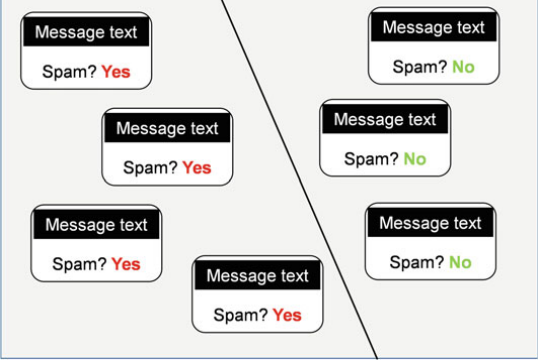
\includegraphics[scale=0.4]{binary-class.png}
	\caption{Ejemplo de clasificación binaria: Identificar si un correo electrónico es spam.}
	\label{fig:bclass}
\end{figure}
\subsection*{Clasificación multi-clase}
Los conjuntos de datos que se usan en clasificación multi-clase son una generalización del caso de clasificación binaria. Solo existe una única variable objetivo, siendo la principal diferencia que esta puede tener cualquier valor dentro de un conjunto valores. Es importante destacar que estos valores son \textbf{discretos} y \textbf{finitos}. El ejemplo más conocido de este tipo de clasificación es la \textbf{clasificación de la flor del Iris}, donde en función de la longitud y anchura del sépalo y del pétalo, se predice si la flor es setosa, virgínica o versicolor.
\begin{figure}[H]
	\centering
	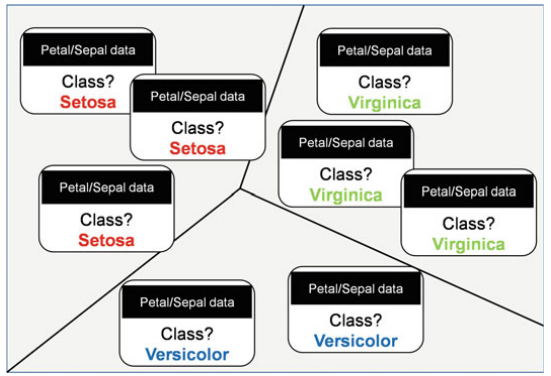
\includegraphics[scale=0.4]{multiclass-class.png}
	\caption{Ejemplo de clasificación multi-clase: Clasificación de la flor del Iris}
	\label{fig:mcclass}
\end{figure}
Muchos de los algoritmos que se usan en Aprendizaje Automático han sido diseñados para clasificación binaria. Con el objetivo de adaptar estos algoritmos existentes a este tipo de problema, existe una técnica llama \textbf{binarización de clase}.
Dos de los enfoques más usados en la actualidad son \textbf{OVA} (\textit{one vs all}) y \textbf{OVO} (\textit{one vs one}). Ambos enfoques tratan de dividir el problema de clasificación multi-clase en varios problemas de clasificación binaria. La diferencia reside en la manera de dividir el problema:
\subsubsection*{One VS All}
Por cada clase, se entrena un clasificador binario donde todas las muestras que pertenecen a la clase seleccionada se selecciona como la clase positiva, el resto como la clase negativa. Una vez que se quiere predecir una nueva muestra, por cada modelo entrenado, se obtiene la probabilidad de que pertenezca a la clase positiva, seleccionando como clase predicha aquella con mayor probabilidad.
\begin{figure}[H]
	\centering
	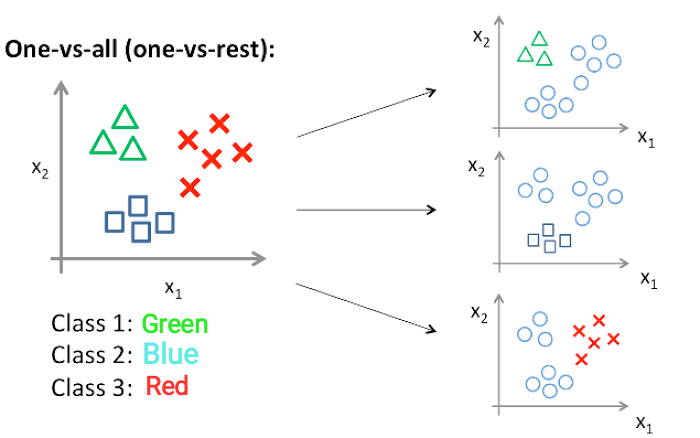
\includegraphics[scale=0.4]{ova.png}
	\caption{Ejemplo de One vs All}
	\label{fig:ova}
\end{figure}
\subsubsection*{One VS One}
A diferencia de \textit{OVA}, por cada par distinto de clases, se entrena un clasificador binario usando una como positiva y otra como negativa. Una vez que llega una nueva muestra, se elige por votación la clase predicha.
\begin{figure}[H]
	\centering
	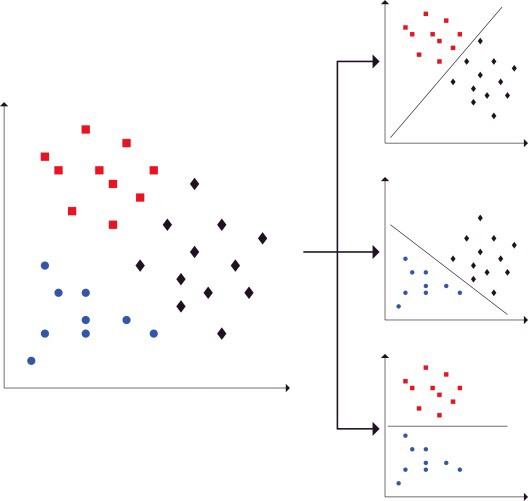
\includegraphics[scale=0.4]{ovo}
	\caption{Ejemplo de One vs One}
	\label{fig:ovo}
\end{figure}
\subsection*{Clasificación ordinal}
Clasificación ordinal es un caso particular de clasificación multi-clase donde existe una relación de orden entre las clases.\\
Un ejemplo de este tipo de clasificación es el de predecir la valoración de una película, predecir las preferencias de una persona (en desacuerdo, de acuerdo).
\subsection*{Clasificación multi-etiqueta}
A diferencia de los anteriores tipos de clasificación, cada muestra tiene un \textbf{conjunto de variables objetivo} en lugar de una única variable. En este caso, el número de variables objetivo es fijo, siendo estas de tipo binario. A cada combinación distinta de valores se conoce como \textit{labelset}.\\
Los algoritmos que usados para este tipo de problema deben de ser capaces de realizar varias predicciones, ya sea modificando los datos originales o adaptando algoritmos de clasificación binaria o multi-clase.\\
\linebreak
Un ejemplo de este tipo de clasificación puede ser el de comprobar si una imagen contiene ciertos elementos.
\begin{figure}[H]
	\centering
	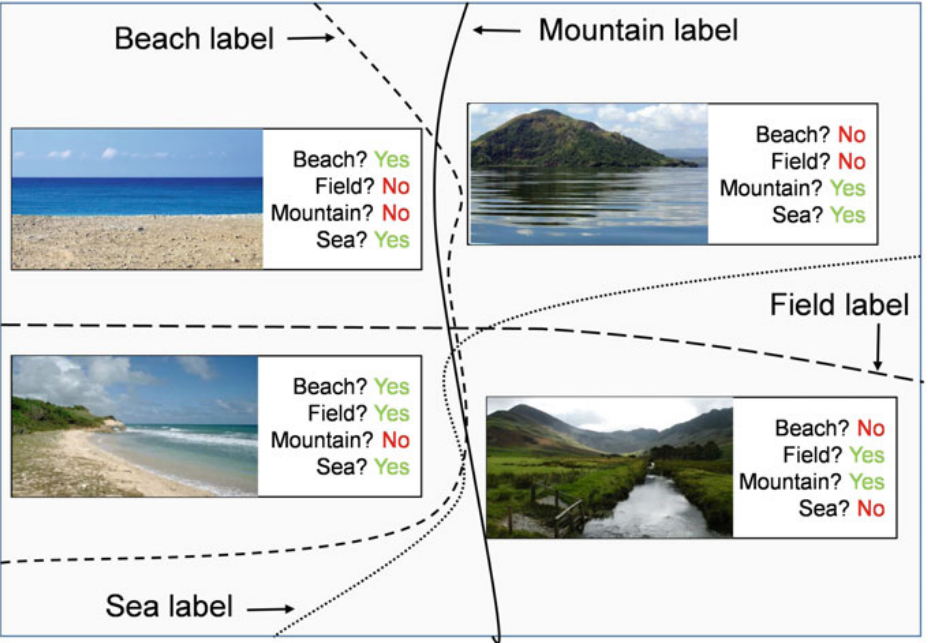
\includegraphics[scale=0.4]{multilabel-class.png}
	\caption{Ejemplo de clasificación multi-etiqueta: Clasificar si una imagen contiene ciertos elementos.}
	\label{fig:mlclasss}
\end{figure}
\subsection*{Clasificación multi-dimensional}
Al igual que la clasificación multi-clase es una generalización del caso binario, la clasificación multi-dimensional es una generalización de la clasificación multi-etiqueta.\\
En este caso, cada muestra tiene un conjunto fijo de variables objetivo que pueden tomar cualquier valor dentro de un conjunto de posibles valores.
\section{Introducción al problema}
Pongámonos en situación de una persona dentro del departamento de marketing de una empresa que se centra en la creación de cursos. Determinar que variables son capaces de definir la intención emprendedora de una sección de la población podría ser beneficioso para la empresa, ya que podrían crear esos cursos enfocándose en aquellas variables más importantes (edad, estudios, ......) para que de una forma más eficiente captar a interesados, cambiar ciertas características de esos cursos para que sean accesibles a gente con más interés y, en definitiva, optimizar los recursos empleados en esos cursos para incrementar el beneficio.\\
\linebreak
Una vez que se ha planteado un objetivo (calcular la intención emprendedora de un conjunto de personas), el siguiente paso es el de elegir como se van a obtener los datos para llegar a ese objetivo. En el caso que se enfoca este trabajo, se ha usado una \textbf{encuesta anónima} sobre un conjunto de personas.
Analizando las preguntas que se hacen en la encuesta. se pueden distinguir tres tipos de preguntas:
\begin{itemize}
	\item \textbf{Variables de control:} Edad, género, estudios, país, etc.
	\item \textbf{Variables de emprendimiento:} Son aquellas que vamos a usar como variables objetivo para los modelos que van a ser usados en las siguientes fases.
	\item\textbf{Variables de competencias:} Estas son las más importantes de cara a los modelos, ya que son las que van a medir el comportamientos del conjunto de personas entrevistadas, dando así información al algoritmo para predecir las \textbf{variables de emprendimiento}.Algunos de estas variables miden \textbf{conocimientos financieros}, \textbf{experiencia}, \textbf{actitudes} que pueden favorecer el carácter emprendedor de un individuo, etc.
\end{itemize}
Con este conjunto de preguntas, se podría obtener un conjunto de datos suficientemente bueno para poder extraer información de los datos. Es importante tener en cuenta que no se está trabajando sobre un conjunto de datos teórico, si no que es un conjunto de datos real, y dependiendo de la forma en la que se haya recogido la información puede ocurrir que se obtengo un conjunto de datos del que no se pueda extraer ninguna información, debido a que tenga un gran nivel de ruido, los datos estén mal muestreados o incluso un mal diseño de la encuesta.\\
\linebreak
La primera fase del proceso de extracción de conocimiento de un conjunto de datos va a ser precisamente esta, haciendo uso de una serie de modelos, se comprobará el rendimiento y se tomará la decisión de si el conjunto de datos es válido o no. En el caso de que todos los modelos seleccionados no funcionen correctamente, se debería de volver a la fase de recolección de datos, con las indicaciones necesarias para lograr un conjunto inicial lo suficientemente bueno. \\
\linebreak
En el caso de que los modelos se comporten bien, el paso seria analizar donde flaquean los algoritmos,  ajustarlos o realizar cambios en el conjunto inicial para incrementar el rendimiento del modelo. A todo este proceso se le conoce como \textbf{KDD} (\textit{Knowledge Discovery in Databases}).
